\batchmode
\documentclass[11pt]{article}
\RequirePackage{ifthen}



\usepackage{graphics} \usepackage{html}

\usepackage{hyperref} \usepackage[usenames, dvipsnames]{color}
\usepackage{colortbl}

\usepackage{sfmath} %
\renewcommand{\familydefault}{\sfdefault}

\markright{PHYS328 Notes}


\setlength{\textwidth} {6.5 true in}  
\setlength{\textheight}{9 true
  in}  
\setlength{\hoffset} {-0.75 true in}  
\setlength{\voffset} {-0.75
  true in}  
\setlength{\parindent} {12 pt}  \pagestyle{myheadings}

\title{PHYS328W Notes} \author{L.A. Riley} \date{Fall 2025}





\makeatletter

\makeatletter
\count@=\the\catcode`\_ \catcode`\_=8 
\newenvironment{tex2html_wrap}{}{}%
\catcode`\<=12\catcode`\_=\count@
\newcommand{\providedcommand}[1]{\expandafter\providecommand\csname #1\endcsname}%
\newcommand{\renewedcommand}[1]{\expandafter\providecommand\csname #1\endcsname{}%
  \expandafter\renewcommand\csname #1\endcsname}%
\newcommand{\newedenvironment}[1]{\newenvironment{#1}{}{}\renewenvironment{#1}}%
\let\newedcommand\renewedcommand
\let\renewedenvironment\newedenvironment
\makeatother
\let\mathon=$
\let\mathoff=$
\ifx\AtBeginDocument\undefined \newcommand{\AtBeginDocument}[1]{}\fi
\newbox\sizebox
\setlength{\hoffset}{0pt}\setlength{\voffset}{0pt}
\addtolength{\textheight}{\footskip}\setlength{\footskip}{0pt}
\addtolength{\textheight}{\topmargin}\setlength{\topmargin}{0pt}
\addtolength{\textheight}{\headheight}\setlength{\headheight}{0pt}
\addtolength{\textheight}{\headsep}\setlength{\headsep}{0pt}
\setlength{\textheight}{504pt}
\newwrite\lthtmlwrite
\makeatletter
\let\realnormalsize=\normalsize
\global\topskip=2sp
\def\preveqno{}\let\real@float=\@float \let\realend@float=\end@float
\def\@float{\let\@savefreelist\@freelist\real@float}
\def\liih@math{\ifmmode$\else\bad@math\fi}
\def\end@float{\realend@float\global\let\@freelist\@savefreelist}
\let\real@dbflt=\@dbflt \let\end@dblfloat=\end@float
\let\@largefloatcheck=\relax
\let\if@boxedmulticols=\iftrue
\def\@dbflt{\let\@savefreelist\@freelist\real@dbflt}
\def\adjustnormalsize{\def\normalsize{\mathsurround=0pt \realnormalsize
 \parindent=0pt\abovedisplayskip=0pt\belowdisplayskip=0pt}%
 \def\phantompar{\csname par\endcsname}\normalsize}%
\def\lthtmltypeout#1{{\let\protect\string \immediate\write\lthtmlwrite{#1}}}%
\usepackage[tightpage,active]{preview}
\PreviewBorder=0.5bp
\newbox\lthtmlPageBox
\newdimen\lthtmlCropMarkHeight
\newdimen\lthtmlCropMarkDepth
\long\def\lthtmlTightVBoxA#1{\def\lthtmllabel{#1}
    \setbox\lthtmlPageBox\vbox\bgroup\catcode`\_=8 }%
\long\def\lthtmlTightVBoxZ{\egroup
    \lthtmlCropMarkHeight=\ht\lthtmlPageBox \advance \lthtmlCropMarkHeight 6pt
    \lthtmlCropMarkDepth=\dp\lthtmlPageBox
    \lthtmltypeout{^^J:\lthtmllabel:lthtmlCropMarkHeight:=\the\lthtmlCropMarkHeight}%
    \lthtmltypeout{^^J:\lthtmllabel:lthtmlCropMarkDepth:=\the\lthtmlCropMarkDepth:1ex:=\the \dimexpr 1ex}%
    \begin{preview}\copy\lthtmlPageBox\end{preview}}%
\long\def\lthtmlTightFBoxA#1{\def\lthtmllabel{#1}%
    \adjustnormalsize\setbox\lthtmlPageBox=\vbox\bgroup\hbox\bgroup %
    \let\ifinner=\iffalse \let\)\liih@math %
    \bgroup\catcode`\_=8 }%
\long\def\lthtmlTightFBoxZ{\egroup\egroup
    \@next\next\@currlist{}{\def\next{\voidb@x}}%
    \expandafter\box\next\egroup %
    \lthtmlCropMarkHeight=\ht\lthtmlPageBox \advance \lthtmlCropMarkHeight 6pt
    \lthtmlCropMarkDepth=\dp\lthtmlPageBox
    \lthtmltypeout{^^J:\lthtmllabel:lthtmlCropMarkHeight:=\the\lthtmlCropMarkHeight}%
    \lthtmltypeout{^^J:\lthtmllabel:lthtmlCropMarkDepth:=\the\lthtmlCropMarkDepth:1ex:=\the \dimexpr 1ex}%
    \begin{preview}\copy\lthtmlPageBox\end{preview}}%
    \long\def\lthtmlinlinemathA#1#2\lthtmlindisplaymathZ{\lthtmlTightVBoxA{#1}{\hbox\bgroup#2\egroup}\lthtmlTightVBoxZ}
    \def\lthtmlinlineA#1#2\lthtmlinlineZ{\lthtmlTightVBoxA{#1}{\hbox\bgroup#2\egroup}\lthtmlTightVBoxZ}
    \long\def\lthtmldisplayA#1#2\lthtmldisplayZ{\lthtmlTightVBoxA{#1}{#2}\lthtmlTightVBoxZ}
    \long\def\lthtmldisplayB#1#2\lthtmldisplayZ{\\edef\preveqno{(\theequation)}%
        \lthtmlTightVBoxA{#1}{\let\@eqnnum\relax#2}\lthtmlTightVBoxZ}
    \long\def\lthtmlfigureA#1{\let\@savefreelist\@freelist
        \lthtmlTightFBoxA{#1}}
    \long\def\lthtmlfigureZ{
        \lthtmlTightFBoxZ\global\let\@freelist\@savefreelist}
    \long\def\lthtmlpictureA#1{\let\@savefreelist\@freelist
        \lthtmlTightVBoxA{#1}}
    \long\def\lthtmlpictureZ{
        \lthtmlTightVBoxZ\global\let\@freelist\@savefreelist}
\def\lthtmlcheckvsize{\ifdim\ht\sizebox<\vsize 
  \ifdim\wd\sizebox<\hsize\expandafter\hfill\fi \expandafter\vfill
  \else\expandafter\vss\fi}%
\providecommand{\selectlanguage}[1]{}%
\makeatletter \tracingstats = 1 


\begin{document}
\pagestyle{empty}\thispagestyle{empty}\lthtmltypeout{}%
\lthtmltypeout{latex2htmlLength hsize=\the\hsize}\lthtmltypeout{}%
\lthtmltypeout{latex2htmlLength vsize=\the\vsize}\lthtmltypeout{}%
\lthtmltypeout{latex2htmlLength hoffset=\the\hoffset}\lthtmltypeout{}%
\lthtmltypeout{latex2htmlLength voffset=\the\voffset}\lthtmltypeout{}%
\lthtmltypeout{latex2htmlLength topmargin=\the\topmargin}\lthtmltypeout{}%
\lthtmltypeout{latex2htmlLength topskip=\the\topskip}\lthtmltypeout{}%
\lthtmltypeout{latex2htmlLength headheight=\the\headheight}\lthtmltypeout{}%
\lthtmltypeout{latex2htmlLength headsep=\the\headsep}\lthtmltypeout{}%
\lthtmltypeout{latex2htmlLength parskip=\the\parskip}\lthtmltypeout{}%
\lthtmltypeout{latex2htmlLength oddsidemargin=\the\oddsidemargin}\lthtmltypeout{}%
\makeatletter
\if@twoside\lthtmltypeout{latex2htmlLength evensidemargin=\the\evensidemargin}%
\else\lthtmltypeout{latex2htmlLength evensidemargin=\the\oddsidemargin}\fi%
\lthtmltypeout{}%
\makeatother
\setcounter{page}{1}
\onecolumn

% !!! IMAGES START HERE !!!

{\newpage\clearpage
\lthtmlinlinemathA{tex2html_wrap_inline3314}%
$Z_1$%
\lthtmlindisplaymathZ
\lthtmlcheckvsize\clearpage}

{\newpage\clearpage
\lthtmlinlinemathA{tex2html_wrap_inline3316}%
$Z_2$%
\lthtmlindisplaymathZ
\lthtmlcheckvsize\clearpage}

{\newpage\clearpage
\lthtmlinlinemathA{tex2html_wrap_inline3320}%
$\omega _o$%
\lthtmlindisplaymathZ
\lthtmlcheckvsize\clearpage}

{\newpage\clearpage
\lthtmlinlinemathA{tex2html_wrap_inline3323}%
$V_{out}/V_{in}$%
\lthtmlindisplaymathZ
\lthtmlcheckvsize\clearpage}

{\newpage\clearpage
\lthtmlinlinemathA{tex2html_wrap_inline3325}%
$\phi $%
\lthtmlindisplaymathZ
\lthtmlcheckvsize\clearpage}

\stepcounter{section}
\stepcounter{subsection}
{\newpage\clearpage
\lthtmlinlinemathA{tex2html_wrap_inline1111}%
$V$%
\lthtmlindisplaymathZ
\lthtmlcheckvsize\clearpage}

{\newpage\clearpage
\lthtmlinlinemathA{tex2html_wrap_inline1113}%
$I$%
\lthtmlindisplaymathZ
\lthtmlcheckvsize\clearpage}

{\newpage\clearpage
\lthtmlinlinemathA{tex2html_wrap_indisplay3334}%
$\displaystyle V=IR
$%
\lthtmlindisplaymathZ
\lthtmlcheckvsize\clearpage}

{\newpage\clearpage
\lthtmlinlinemathA{tex2html_wrap_inline1115}%
$R$%
\lthtmlindisplaymathZ
\lthtmlcheckvsize\clearpage}

{\newpage\clearpage
\lthtmlinlinemathA{tex2html_wrap_indisplay3337}%
$\displaystyle P_\mathrm{diss} = I^2 R = \frac{V^2}{R}
$%
\lthtmlindisplaymathZ
\lthtmlcheckvsize\clearpage}

\stepcounter{subsection}
{\newpage\clearpage
\lthtmlfigureA{figure46}%
\begin{figure}  \htmlimage{align='center'}{}
  \begin{center}
    \includegraphics{seriesparallel.eps}
    
  \end{center}
\end{figure}%
\lthtmlfigureZ
\lthtmlcheckvsize\clearpage}

{\newpage\clearpage
\lthtmlinlinemathA{tex2html_wrap_inline1117}%
$R_\mathrm{eq}$%
\lthtmlindisplaymathZ
\lthtmlcheckvsize\clearpage}

{\newpage\clearpage
\lthtmlinlinemathA{tex2html_wrap_indisplay3344}%
$\displaystyle R_{eq} = R_1 + R_2 + R_3 + \ldots
$%
\lthtmlindisplaymathZ
\lthtmlcheckvsize\clearpage}

{\newpage\clearpage
\lthtmlinlinemathA{tex2html_wrap_indisplay3346}%
$\displaystyle \frac{1}{R_{eq}} = \frac{1}{R_1} + \frac{1}{R_2} + \frac{1}{R_3} +
  \ldots
$%
\lthtmlindisplaymathZ
\lthtmlcheckvsize\clearpage}

{\newpage\clearpage
\lthtmlinlinemathA{tex2html_wrap_inline1119}%
$R_1||R_2||R_3...$%
\lthtmlindisplaymathZ
\lthtmlcheckvsize\clearpage}

{\newpage\clearpage
\lthtmlinlinemathA{tex2html_wrap_indisplay3350}%
$\displaystyle
  V_1 = \frac{R_1}{R_1 + R_2} V
$%
\lthtmlindisplaymathZ
\lthtmlcheckvsize\clearpage}

{\newpage\clearpage
\lthtmlinlinemathA{tex2html_wrap_indisplay3352}%
$\displaystyle
  V_2 = \frac{R_2}{R_1 + R_2} V
$%
\lthtmlindisplaymathZ
\lthtmlcheckvsize\clearpage}

{\newpage\clearpage
\lthtmlinlinemathA{tex2html_wrap_indisplay3355}%
$\displaystyle
  I_1 = \frac{R_2}{R_1 + R_2} I
$%
\lthtmlindisplaymathZ
\lthtmlcheckvsize\clearpage}

{\newpage\clearpage
\lthtmlinlinemathA{tex2html_wrap_indisplay3357}%
$\displaystyle
  I_2 = \frac{R_1}{R_1 + R_2} I
$%
\lthtmlindisplaymathZ
\lthtmlcheckvsize\clearpage}

{\newpage\clearpage
\lthtmlinlinemathA{tex2html_wrap_inline1125}%
$I_1$%
\lthtmlindisplaymathZ
\lthtmlcheckvsize\clearpage}

{\newpage\clearpage
\lthtmlinlinemathA{tex2html_wrap_inline1127}%
$R_1$%
\lthtmlindisplaymathZ
\lthtmlcheckvsize\clearpage}

{\newpage\clearpage
\lthtmlinlinemathA{tex2html_wrap_inline1129}%
$I_2$%
\lthtmlindisplaymathZ
\lthtmlcheckvsize\clearpage}

{\newpage\clearpage
\lthtmlinlinemathA{tex2html_wrap_inline1131}%
$R_2$%
\lthtmlindisplaymathZ
\lthtmlcheckvsize\clearpage}

\stepcounter{subsection}
{\newpage\clearpage
\lthtmlfigureA{figure102}%
\begin{figure}  \htmlimage{align='center'}{}
  \begin{center}
    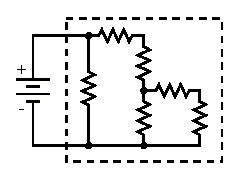
\includegraphics{rnetwork.eps}
    
  \end{center}
\end{figure}%
\lthtmlfigureZ
\lthtmlcheckvsize\clearpage}

{\newpage\clearpage
\lthtmlinlinemathA{tex2html_wrap_inline1133}%
$\Delta$%
\lthtmlindisplaymathZ
\lthtmlcheckvsize\clearpage}

{\newpage\clearpage
\lthtmlinlinemathA{tex2html_wrap_inline1135}%
$\bullet$%
\lthtmlindisplaymathZ
\lthtmlcheckvsize\clearpage}

{\newpage\clearpage
\lthtmlinlinemathA{tex2html_wrap_inline1139}%
$Y$%
\lthtmlindisplaymathZ
\lthtmlcheckvsize\clearpage}

{\newpage\clearpage
\lthtmlinlinemathA{tex2html_wrap_inline1141}%
$\Delta-Y$%
\lthtmlindisplaymathZ
\lthtmlcheckvsize\clearpage}

\stepcounter{subsection}
{\newpage\clearpage
\lthtmlinlinemathA{tex2html_wrap_indisplay3374}%
$\displaystyle \sum_\mathrm{loop} V_i = 0
$%
\lthtmlindisplaymathZ
\lthtmlcheckvsize\clearpage}

{\newpage\clearpage
\lthtmlinlinemathA{tex2html_wrap_inline1143}%
$V_i$%
\lthtmlindisplaymathZ
\lthtmlcheckvsize\clearpage}

{\newpage\clearpage
\lthtmlfigureA{figure131}%
\begin{figure}  \begin{center}
    \htmlimage{align='center'}{} 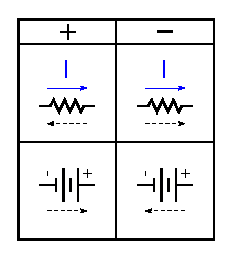
\includegraphics{kirchhoffsigns.eps}
    
  \end{center}
\end{figure}%
\lthtmlfigureZ
\lthtmlcheckvsize\clearpage}

{\newpage\clearpage
\lthtmlinlinemathA{tex2html_wrap_indisplay3380}%
$\displaystyle \sum_\mathrm{junction} I_i = 0
$%
\lthtmlindisplaymathZ
\lthtmlcheckvsize\clearpage}

\stepcounter{subsection}
{\newpage\clearpage
\lthtmlfigureA{figure150}%
\begin{figure}  \begin{center}
    \htmlimage{align='center'}{} 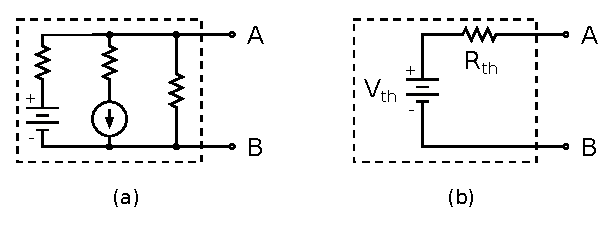
\includegraphics{thevenin.eps}
    
  \end{center}
\end{figure}%
\lthtmlfigureZ
\lthtmlcheckvsize\clearpage}

{\newpage\clearpage
\lthtmlinlinemathA{tex2html_wrap_inline1145}%
$V_{th}$%
\lthtmlindisplaymathZ
\lthtmlcheckvsize\clearpage}

{\newpage\clearpage
\lthtmlinlinemathA{tex2html_wrap_inline1147}%
$A$%
\lthtmlindisplaymathZ
\lthtmlcheckvsize\clearpage}

{\newpage\clearpage
\lthtmlinlinemathA{tex2html_wrap_inline1149}%
$B$%
\lthtmlindisplaymathZ
\lthtmlcheckvsize\clearpage}

{\newpage\clearpage
\lthtmlinlinemathA{tex2html_wrap_inline1151}%
$R_{th}$%
\lthtmlindisplaymathZ
\lthtmlcheckvsize\clearpage}

\stepcounter{section}
\stepcounter{subsection}
{\newpage\clearpage
\lthtmlinlinemathA{tex2html_wrap_inline1157}%
$\pi/2$%
\lthtmlindisplaymathZ
\lthtmlcheckvsize\clearpage}

{\newpage\clearpage
\lthtmlinlinemathA{tex2html_wrap_indisplay3398}%
$\displaystyle X_L = j \omega L
$%
\lthtmlindisplaymathZ
\lthtmlcheckvsize\clearpage}

{\newpage\clearpage
\lthtmlinlinemathA{tex2html_wrap_inline1161}%
$\omega = 2 \pi f$%
\lthtmlindisplaymathZ
\lthtmlcheckvsize\clearpage}

{\newpage\clearpage
\lthtmlinlinemathA{tex2html_wrap_inline1163}%
$L$%
\lthtmlindisplaymathZ
\lthtmlcheckvsize\clearpage}

{\newpage\clearpage
\lthtmlinlinemathA{tex2html_wrap_inline1165}%
$j$%
\lthtmlindisplaymathZ
\lthtmlcheckvsize\clearpage}

{\newpage\clearpage
\lthtmlinlinemathA{tex2html_wrap_inline1167}%
$\sqrt{-1}$%
\lthtmlindisplaymathZ
\lthtmlcheckvsize\clearpage}

{\newpage\clearpage
\lthtmlinlinemathA{tex2html_wrap_inline1169}%
$i$%
\lthtmlindisplaymathZ
\lthtmlcheckvsize\clearpage}

{\newpage\clearpage
\lthtmlinlinemathA{tex2html_wrap_indisplay3405}%
$\displaystyle X_C = -\frac{j}{\omega C}
$%
\lthtmlindisplaymathZ
\lthtmlcheckvsize\clearpage}

{\newpage\clearpage
\lthtmlinlinemathA{tex2html_wrap_inline1171}%
$C$%
\lthtmlindisplaymathZ
\lthtmlcheckvsize\clearpage}

{\newpage\clearpage
\lthtmlinlinemathA{tex2html_wrap_inline1175}%
$Z$%
\lthtmlindisplaymathZ
\lthtmlcheckvsize\clearpage}

\stepcounter{subsection}
{\newpage\clearpage
\lthtmlinlinemathA{tex2html_wrap_indisplay3413}%
$\displaystyle v(t)$%
\lthtmlindisplaymathZ
\lthtmlcheckvsize\clearpage}

{\newpage\clearpage
\lthtmlinlinemathA{tex2html_wrap_indisplay3414}%
$\textstyle =$%
\lthtmlindisplaymathZ
\lthtmlcheckvsize\clearpage}

{\newpage\clearpage
\lthtmlinlinemathA{tex2html_wrap_indisplay3415}%
$\displaystyle Re \left(V \, e^{\,j(\omega t + \phi_v}) \right) = V
\cos(\omega t + \phi_v)$%
\lthtmlindisplaymathZ
\lthtmlcheckvsize\clearpage}

{\newpage\clearpage
\lthtmlinlinemathA{tex2html_wrap_indisplay3416}%
$\displaystyle i(t)$%
\lthtmlindisplaymathZ
\lthtmlcheckvsize\clearpage}

{\newpage\clearpage
\lthtmlinlinemathA{tex2html_wrap_indisplay3418}%
$\displaystyle Re \left(I \,
e^{\,j(\omega t + \phi_i)} \right) = I \cos(\omega t + \phi_i)$%
\lthtmlindisplaymathZ
\lthtmlcheckvsize\clearpage}

{\newpage\clearpage
\lthtmlinlinemathA{tex2html_wrap_inline1185}%
$\phi_i$%
\lthtmlindisplaymathZ
\lthtmlcheckvsize\clearpage}

{\newpage\clearpage
\lthtmlinlinemathA{tex2html_wrap_inline1187}%
$\phi_v$%
\lthtmlindisplaymathZ
\lthtmlcheckvsize\clearpage}

{\newpage\clearpage
\lthtmlinlinemathA{tex2html_wrap_inline1189}%
$e^{j \omega t}$%
\lthtmlindisplaymathZ
\lthtmlcheckvsize\clearpage}

{\newpage\clearpage
\lthtmlinlinemathA{tex2html_wrap_indisplay3425}%
$\displaystyle \mathbf{V}$%
\lthtmlindisplaymathZ
\lthtmlcheckvsize\clearpage}

{\newpage\clearpage
\lthtmlinlinemathA{tex2html_wrap_indisplay3427}%
$\displaystyle V \, e^{\,j \phi_v}$%
\lthtmlindisplaymathZ
\lthtmlcheckvsize\clearpage}

{\newpage\clearpage
\lthtmlinlinemathA{tex2html_wrap_indisplay3428}%
$\displaystyle \mathbf{I}$%
\lthtmlindisplaymathZ
\lthtmlcheckvsize\clearpage}

{\newpage\clearpage
\lthtmlinlinemathA{tex2html_wrap_indisplay3430}%
$\displaystyle I \,
e^{\,j \phi_i}$%
\lthtmlindisplaymathZ
\lthtmlcheckvsize\clearpage}

{\newpage\clearpage
\lthtmlinlinemathA{tex2html_wrap_indisplay3434}%
$\displaystyle Re(\mathbf{V} \, e^{\,j\omega t})$%
\lthtmlindisplaymathZ
\lthtmlcheckvsize\clearpage}

{\newpage\clearpage
\lthtmlinlinemathA{tex2html_wrap_indisplay3437}%
$\displaystyle Re(\mathbf{I} \, e^{\,j\omega t})$%
\lthtmlindisplaymathZ
\lthtmlcheckvsize\clearpage}

{\newpage\clearpage
\lthtmlinlinemathA{tex2html_wrap_indisplay3439}%
$\displaystyle \mathbf{I} = \frac{\mathbf{V}}{Z}
$%
\lthtmlindisplaymathZ
\lthtmlcheckvsize\clearpage}

{\newpage\clearpage
\lthtmlinlinemathA{tex2html_wrap_indisplay3441}%
$\displaystyle \mathbf{P} = \mathbf{I^*V} = IV \, e^{\,j(\phi_v - \phi_i)}
$%
\lthtmlindisplaymathZ
\lthtmlcheckvsize\clearpage}

{\newpage\clearpage
\lthtmlinlinemathA{tex2html_wrap_indisplay3443}%
$\displaystyle \left< P \right> = \frac{IV}{2} \cos(\phi_v - \phi_i) =
  \frac{V^2}{2Z} \cos(\phi_v - \phi_i)
$%
\lthtmlindisplaymathZ
\lthtmlcheckvsize\clearpage}

{\newpage\clearpage
\lthtmlinlinemathA{tex2html_wrap_inline1191}%
$\cos^2(\omega t)$%
\lthtmlindisplaymathZ
\lthtmlcheckvsize\clearpage}

{\newpage\clearpage
\lthtmlinlinemathA{tex2html_wrap_inline1193}%
$\phi_v - \phi_i$%
\lthtmlindisplaymathZ
\lthtmlcheckvsize\clearpage}

{\newpage\clearpage
\lthtmlinlinemathA{tex2html_wrap_inline1197}%
$-\pi/2$%
\lthtmlindisplaymathZ
\lthtmlcheckvsize\clearpage}

{\newpage\clearpage
\lthtmlinlinemathA{tex2html_wrap_inline1199}%
$\mathbf{V}$%
\lthtmlindisplaymathZ
\lthtmlcheckvsize\clearpage}

{\newpage\clearpage
\lthtmlinlinemathA{tex2html_wrap_inline1201}%
$\mathbf{I}$%
\lthtmlindisplaymathZ
\lthtmlcheckvsize\clearpage}

\stepcounter{subsection}
{\newpage\clearpage
\lthtmlfigureA{figure247}%
\begin{figure}  \begin{center}
    \htmlimage{align='center'}{} 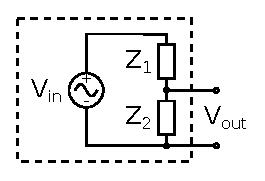
\includegraphics{acvdivider.eps}
    
  \end{center}
\end{figure}%
\lthtmlfigureZ
\lthtmlcheckvsize\clearpage}

{\newpage\clearpage
\lthtmlinlinemathA{tex2html_wrap_indisplay3463}%
$\displaystyle \mathbf{V_{in}} - \mathbf{I} Z_1 - \mathbf{I} Z_2 = 0
$%
\lthtmlindisplaymathZ
\lthtmlcheckvsize\clearpage}

{\newpage\clearpage
\lthtmlinlinemathA{tex2html_wrap_indisplay3466}%
$\displaystyle \mathbf{V_{out}} = \mathbf{I} Z_2
$%
\lthtmlindisplaymathZ
\lthtmlcheckvsize\clearpage}

{\newpage\clearpage
\lthtmlinlinemathA{tex2html_wrap_indisplay3468}%
$\displaystyle \mathbf{V_{out}} = \frac{Z_2}{Z_1 + Z_2} \mathbf{V_{in}}
$%
\lthtmlindisplaymathZ
\lthtmlcheckvsize\clearpage}

{\newpage\clearpage
\lthtmlinlinemathA{tex2html_wrap_inline1215}%
$\mathbf{V_{out}}$%
\lthtmlindisplaymathZ
\lthtmlcheckvsize\clearpage}

{\newpage\clearpage
\lthtmlinlinemathA{tex2html_wrap_indisplay3471}%
$\displaystyle V_{out} = \sqrt{\mathbf{V_{out}^* V_{out}}}
$%
\lthtmlindisplaymathZ
\lthtmlcheckvsize\clearpage}

{\newpage\clearpage
\lthtmlinlinemathA{tex2html_wrap_inline1221}%
$\mathbf{V_{in}}$%
\lthtmlindisplaymathZ
\lthtmlcheckvsize\clearpage}

{\newpage\clearpage
\lthtmlinlinemathA{tex2html_wrap_indisplay3480}%
$\displaystyle \tan \phi = \frac{ Im \left( \frac{Z_2}{Z_1 + Z_2} \right) } { Re
    \left( \frac{Z_2}{Z_1 + Z_2} \right) }
$%
\lthtmlindisplaymathZ
\lthtmlcheckvsize\clearpage}

{\newpage\clearpage
\lthtmlinlinemathA{tex2html_wrap_inline1233}%
$A_V$%
\lthtmlindisplaymathZ
\lthtmlcheckvsize\clearpage}

{\newpage\clearpage
\lthtmlinlinemathA{tex2html_wrap_indisplay3487}%
$\displaystyle A_V = \frac{V_{out}}{V_{in}} =
  \frac{|\mathbf{V_{out}}|}{|\mathbf{V_{in}}|} = \left| \frac{Z_2}{Z_1
    + Z_2} \right| = \sqrt{ \left( \frac{Z_2}{Z_1 + Z_2} \right)^*
    \left( \frac{Z_2}{Z_1 + Z_2} \right) }
$%
\lthtmlindisplaymathZ
\lthtmlcheckvsize\clearpage}

{\newpage\clearpage
\lthtmlinlinemathA{tex2html_wrap_inline1237}%
$\frac{1}{2}$%
\lthtmlindisplaymathZ
\lthtmlcheckvsize\clearpage}

{\newpage\clearpage
\lthtmlinlinemathA{tex2html_wrap_inline1239}%
$A_v = \frac{1}{\sqrt{2}}$%
\lthtmlindisplaymathZ
\lthtmlcheckvsize\clearpage}

{\newpage\clearpage
\lthtmlfigureA{figure327}%
\begin{figure}  \begin{center}
    \htmlimage{align='center'}{} 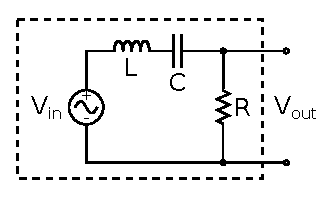
\includegraphics{rlccircuit.eps}
    
  \end{center}
\end{figure}%
\lthtmlfigureZ
\lthtmlcheckvsize\clearpage}

{\newpage\clearpage
\lthtmlinlinemathA{tex2html_wrap_inline1241}%
$Z_2 = R$%
\lthtmlindisplaymathZ
\lthtmlcheckvsize\clearpage}

{\newpage\clearpage
\lthtmlinlinemathA{tex2html_wrap_indisplay3496}%
$\displaystyle Z_1 = j \left( \omega L - \frac{1}{\omega C} \right)
$%
\lthtmlindisplaymathZ
\lthtmlcheckvsize\clearpage}

{\newpage\clearpage
\lthtmlinlinemathA{tex2html_wrap_indisplay3498}%
$\displaystyle \frac{V_{out}}{V_{in}} = \sqrt{\frac{R^2}{R^2 + (\omega L - 1/\omega
      C)^2}}
$%
\lthtmlindisplaymathZ
\lthtmlcheckvsize\clearpage}

{\newpage\clearpage
\lthtmlinlinemathA{tex2html_wrap_inline1243}%
$a + jb$%
\lthtmlindisplaymathZ
\lthtmlcheckvsize\clearpage}

{\newpage\clearpage
\lthtmlinlinemathA{tex2html_wrap_indisplay3501}%
$\displaystyle \frac{Z_2}{Z_1 + Z_2} = \frac{R}{R + j \left( \omega L -
    \frac{1}{\omega C} \right)} = \frac{R^2 - j R \left( \omega L -
    \frac{1}{\omega C} \right)} {R^2 + \left( \omega L -
    \frac{1}{\omega C} \right)^2}
$%
\lthtmlindisplaymathZ
\lthtmlcheckvsize\clearpage}

{\newpage\clearpage
\lthtmlinlinemathA{tex2html_wrap_indisplay3503}%
$\displaystyle \tan \phi = \frac{\frac{1}{\omega C} - \omega L}{R}
$%
\lthtmlindisplaymathZ
\lthtmlcheckvsize\clearpage}

{\newpage\clearpage
\lthtmlinlinemathA{tex2html_wrap_inline1245}%
$v_{out}(t)$%
\lthtmlindisplaymathZ
\lthtmlcheckvsize\clearpage}

{\newpage\clearpage
\lthtmlinlinemathA{tex2html_wrap_inline1247}%
$v_{in}(t)$%
\lthtmlindisplaymathZ
\lthtmlcheckvsize\clearpage}

{\newpage\clearpage
\lthtmlinlinemathA{tex2html_wrap_inline1251}%
$\Delta t = t_{V_{out}} -
t_{V_{in}}$%
\lthtmlindisplaymathZ
\lthtmlcheckvsize\clearpage}

{\newpage\clearpage
\lthtmlinlinemathA{tex2html_wrap_indisplay3509}%
$\displaystyle \Delta t = -\frac{\phi}{\omega} = -\frac{\phi}{2 \pi f} =
  -\frac{\phi}{2 \pi} T
$%
\lthtmlindisplaymathZ
\lthtmlcheckvsize\clearpage}

{\newpage\clearpage
\lthtmlinlinemathA{tex2html_wrap_inline1253}%
$T$%
\lthtmlindisplaymathZ
\lthtmlcheckvsize\clearpage}

{\newpage\clearpage
\lthtmlinlinemathA{tex2html_wrap_inline1255}%
$V_{out}$%
\lthtmlindisplaymathZ
\lthtmlcheckvsize\clearpage}

{\newpage\clearpage
\lthtmlinlinemathA{tex2html_wrap_inline1257}%
$V_{in}$%
\lthtmlindisplaymathZ
\lthtmlcheckvsize\clearpage}

{\newpage\clearpage
\lthtmlfigureA{figure385}%
\begin{figure}  \htmlimage{align='center'}{}
  \begin{center}
    \scalebox{0.45}{ 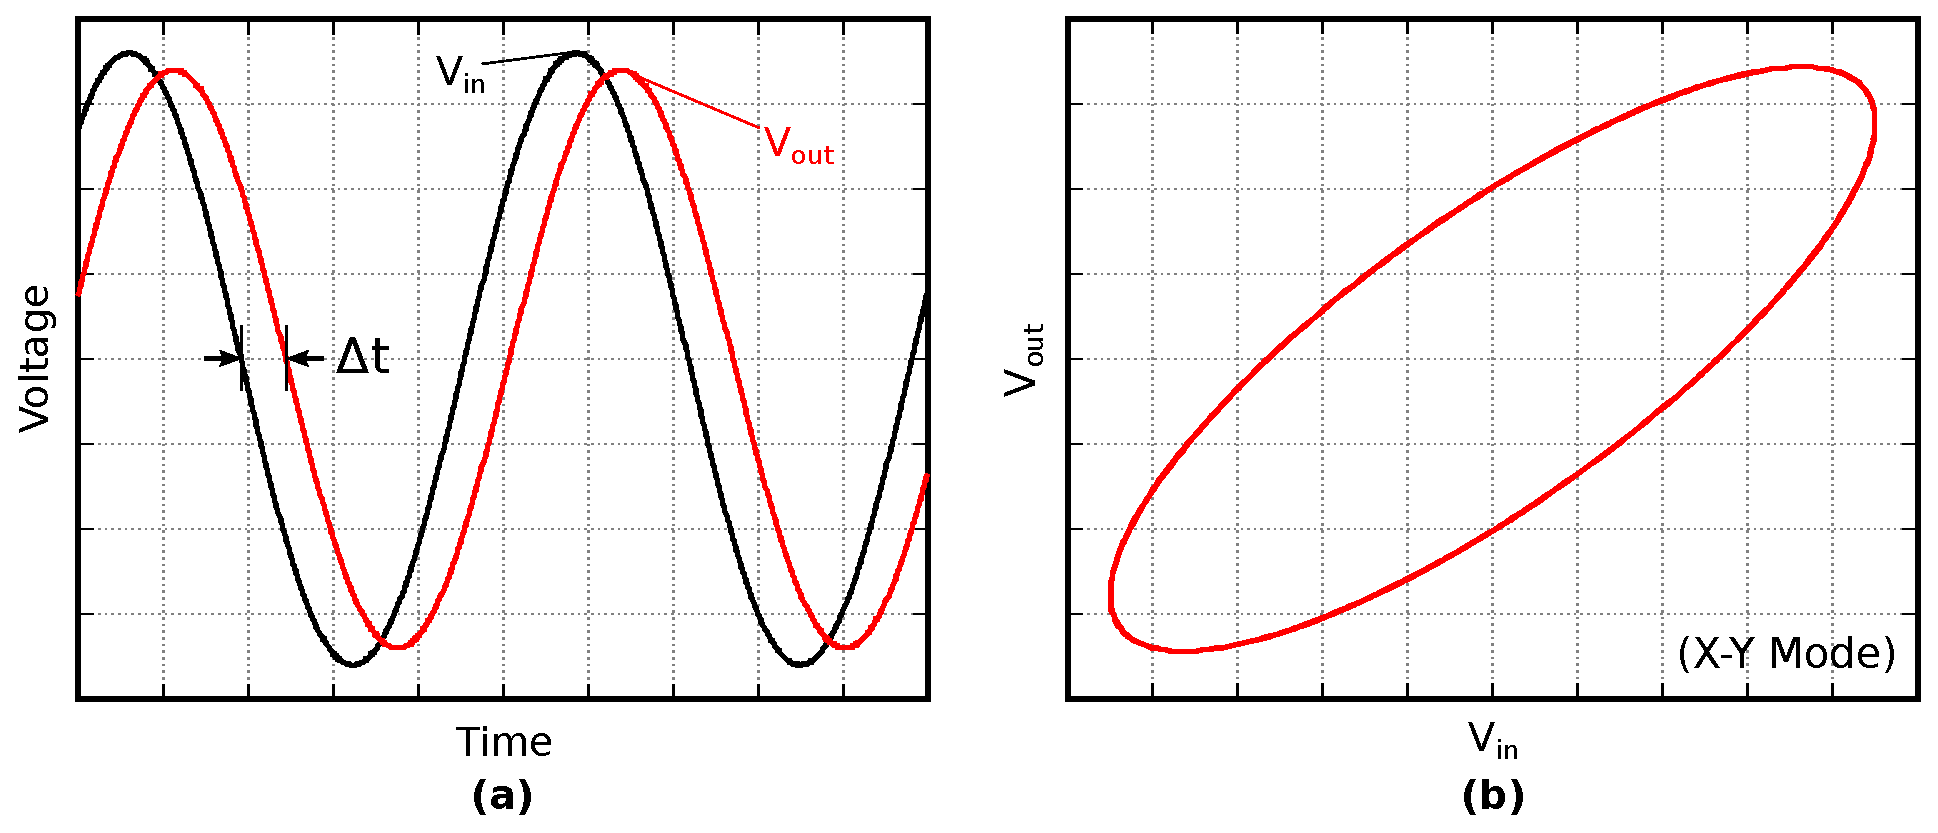
\includegraphics{rlcnr.eps} }
    \vspace{12 pt} \scalebox{0.45}{ 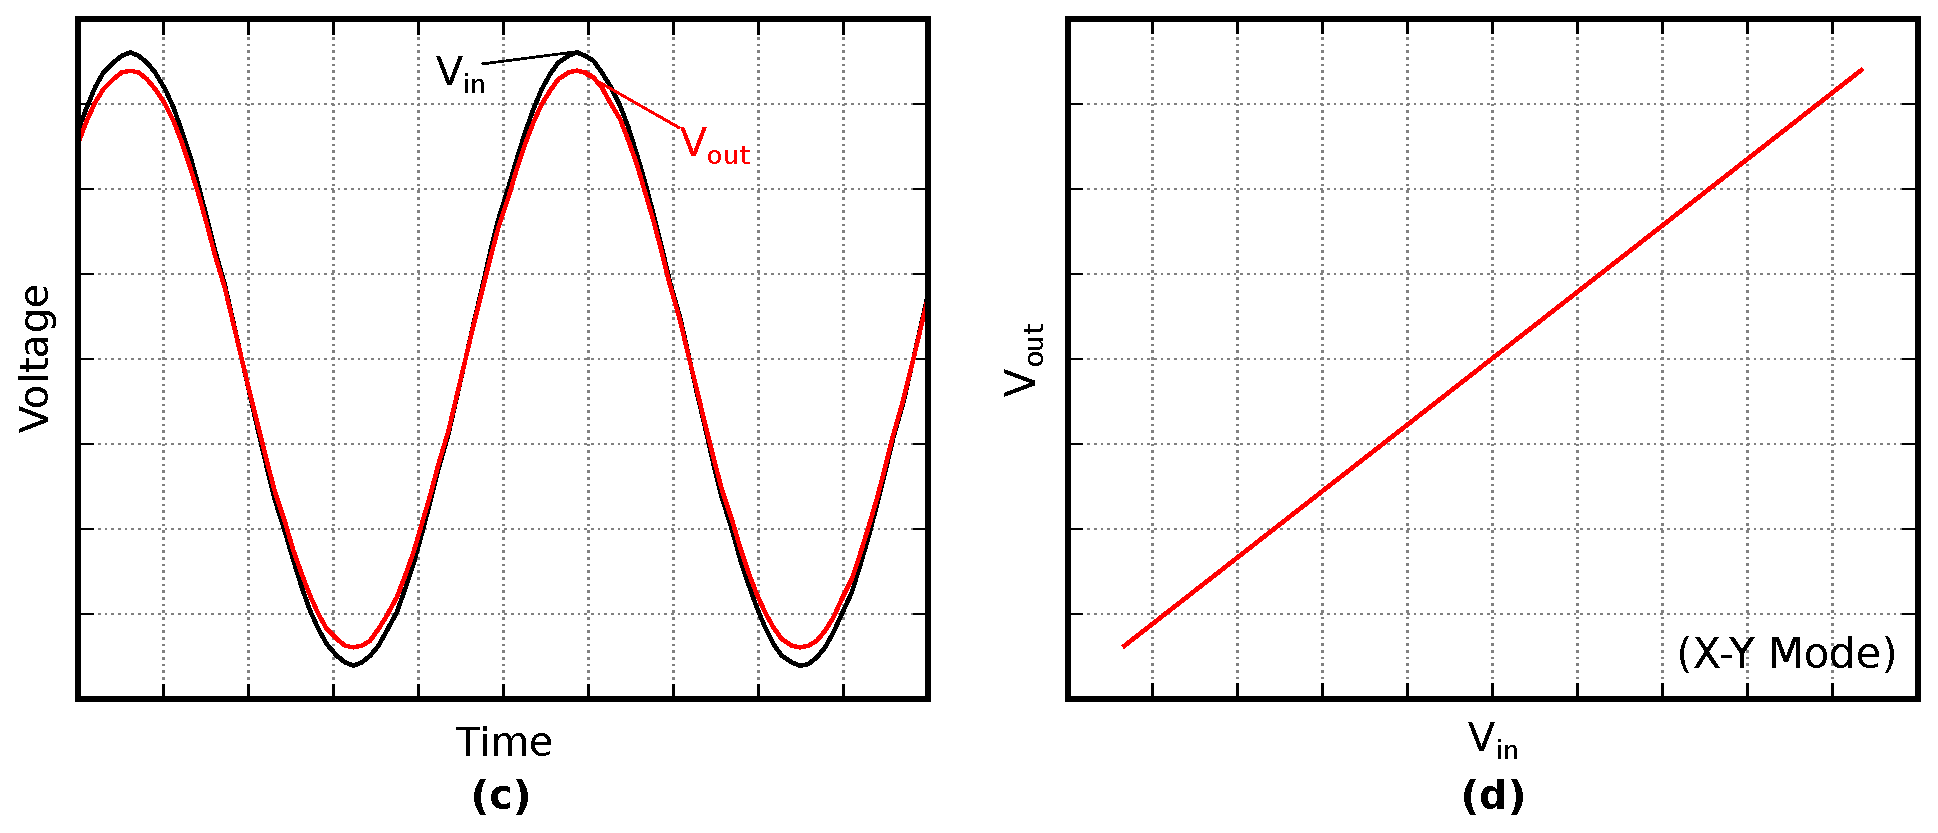
\includegraphics{rlcres.eps} }
    
  \end{center}
\end{figure}%
\lthtmlfigureZ
\lthtmlcheckvsize\clearpage}

{\newpage\clearpage
\lthtmlfigureA{figure398}%
\begin{figure}  \htmlimage{align='center'}{}
  \begin{center}
    \scalebox{0.45}{ 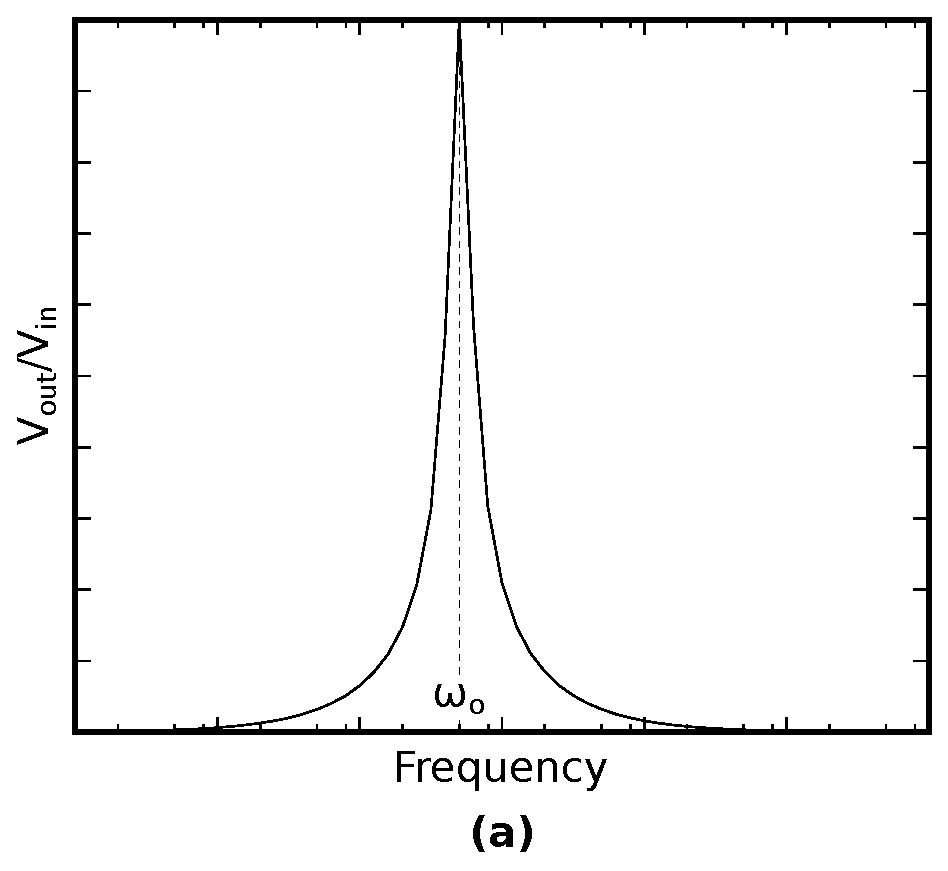
\includegraphics{rlc_vout.eps} }
    \hspace{12 pt} \scalebox{0.45}{ 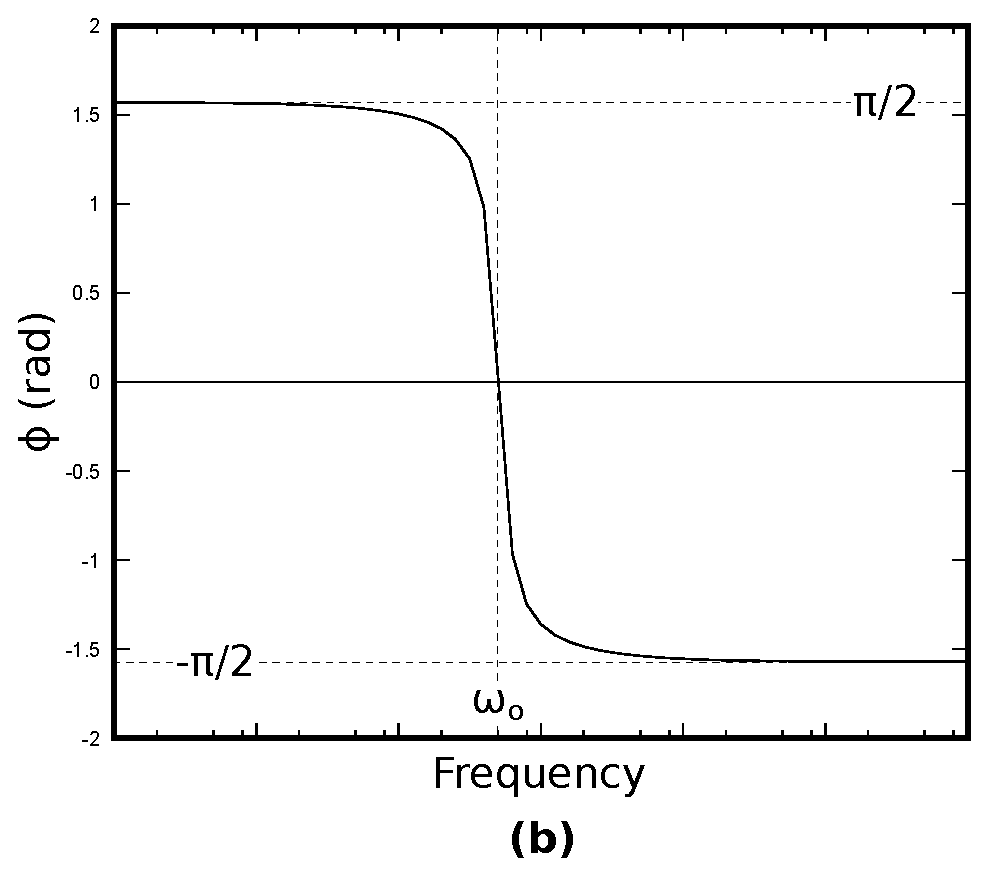
\includegraphics{rlc_phi.eps} }
    
  \end{center}
\end{figure}%
\lthtmlfigureZ
\lthtmlcheckvsize\clearpage}

{\newpage\clearpage
\lthtmlinlinemathA{tex2html_wrap_inline1271}%
$V_{out} = V_{in}$%
\lthtmlindisplaymathZ
\lthtmlcheckvsize\clearpage}

{\newpage\clearpage
\lthtmlinlinemathA{tex2html_wrap_inline1275}%
$X_L$%
\lthtmlindisplaymathZ
\lthtmlcheckvsize\clearpage}

{\newpage\clearpage
\lthtmlinlinemathA{tex2html_wrap_inline1277}%
$X_C$%
\lthtmlindisplaymathZ
\lthtmlcheckvsize\clearpage}

{\newpage\clearpage
\lthtmlinlinemathA{tex2html_wrap_indisplay3533}%
$\displaystyle \omega_o = \frac{1}{\sqrt{LC}}
$%
\lthtmlindisplaymathZ
\lthtmlcheckvsize\clearpage}

{\newpage\clearpage
\lthtmlinlinemathA{tex2html_wrap_inline1287}%
$A_V = V_{out}/V_{in}$%
\lthtmlindisplaymathZ
\lthtmlcheckvsize\clearpage}

{\newpage\clearpage
\lthtmlinlinemathA{tex2html_wrap_inline1291}%
$v_{out}$%
\lthtmlindisplaymathZ
\lthtmlcheckvsize\clearpage}

\stepcounter{section}
{\newpage\clearpage
\lthtmlfigureA{figure442}%
\begin{figure}  \htmlimage{align='center'}{}
  \begin{center}
    \scalebox{0.5}{ 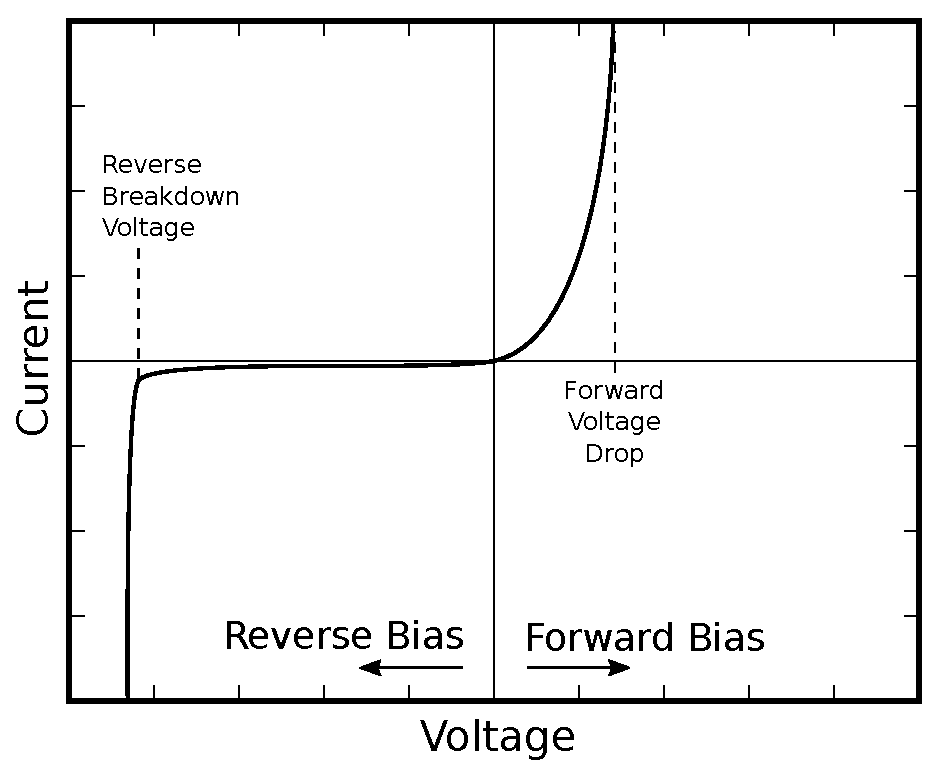
\includegraphics{diodevi.eps} }
    
  \end{center}
\end{figure}%
\lthtmlfigureZ
\lthtmlcheckvsize\clearpage}

{\newpage\clearpage
\lthtmlinlinemathA{tex2html_wrap_inline1297}%
$V-I$%
\lthtmlindisplaymathZ
\lthtmlcheckvsize\clearpage}

{\newpage\clearpage
\lthtmlinlinemathA{tex2html_wrap_inline1299}%
$10^{-8}$%
\lthtmlindisplaymathZ
\lthtmlcheckvsize\clearpage}

{\newpage\clearpage
\lthtmlpictureA{tex2html_wrap3549}%
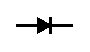
\includegraphics{diode.eps}%
\lthtmlpictureZ
\lthtmlcheckvsize\clearpage}

\stepcounter{section}
{\newpage\clearpage
\lthtmlfigureA{figure464}%
\begin{figure}  \htmlimage{align='center'}{}
  \begin{center}
    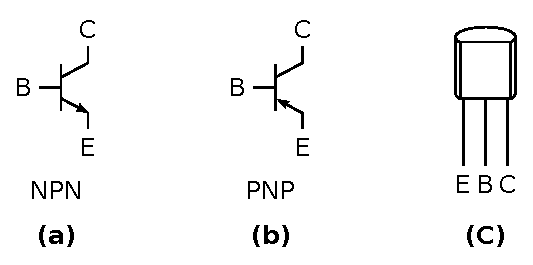
\includegraphics{transistors.eps}
    
  \end{center}
\end{figure}%
\lthtmlfigureZ
\lthtmlcheckvsize\clearpage}

{\newpage\clearpage
\lthtmlinlinemathA{tex2html_wrap_inline1301}%
$I_C$%
\lthtmlindisplaymathZ
\lthtmlcheckvsize\clearpage}

\stepcounter{subsection}
{\newpage\clearpage
\lthtmlinlinemathA{tex2html_wrap_inline1305}%
$V_{BE}$%
\lthtmlindisplaymathZ
\lthtmlcheckvsize\clearpage}

{\newpage\clearpage
\lthtmlinlinemathA{tex2html_wrap_indisplay3560}%
$\displaystyle I_C = I_o \left( e^{\frac{V_{BE}}{kT/e}} - 1 \right)
$%
\lthtmlindisplaymathZ
\lthtmlcheckvsize\clearpage}

{\newpage\clearpage
\lthtmlinlinemathA{tex2html_wrap_inline1307}%
$I_o$%
\lthtmlindisplaymathZ
\lthtmlcheckvsize\clearpage}

{\newpage\clearpage
\lthtmlinlinemathA{tex2html_wrap_inline1309}%
$e = 1.6 \times 10^{-19}$%
\lthtmlindisplaymathZ
\lthtmlcheckvsize\clearpage}

{\newpage\clearpage
\lthtmlinlinemathA{tex2html_wrap_inline1311}%
$k
= 1.38 \times 10^{-23}$%
\lthtmlindisplaymathZ
\lthtmlcheckvsize\clearpage}

{\newpage\clearpage
\lthtmlfigureA{figure492}%
\begin{figure}  \htmlimage{align='center'}{}
  \begin{center}
    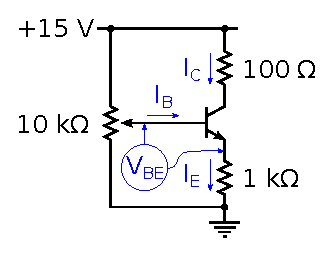
\includegraphics{ebersmollcircuit.eps}
    
  \end{center}
\end{figure}%
\lthtmlfigureZ
\lthtmlcheckvsize\clearpage}

{\newpage\clearpage
\lthtmlinlinemathA{tex2html_wrap_inline1321}%
$\approx
0.7$%
\lthtmlindisplaymathZ
\lthtmlcheckvsize\clearpage}

{\newpage\clearpage
\lthtmlinlinemathA{tex2html_wrap_inline1325}%
$\Omega$%
\lthtmlindisplaymathZ
\lthtmlcheckvsize\clearpage}

{\newpage\clearpage
\lthtmlinlinemathA{tex2html_wrap_indisplay3579}%
$\displaystyle r_e = \frac{d V_{BE}}{d I_C} = \frac{kT/e}{I_C}
$%
\lthtmlindisplaymathZ
\lthtmlcheckvsize\clearpage}

{\newpage\clearpage
\lthtmlinlinemathA{tex2html_wrap_inline1335}%
$(25~\Omega)/I_C[\mathrm{mA}]$%
\lthtmlindisplaymathZ
\lthtmlcheckvsize\clearpage}

{\newpage\clearpage
\lthtmlinlinemathA{tex2html_wrap_inline1337}%
$V_{CE}$%
\lthtmlindisplaymathZ
\lthtmlcheckvsize\clearpage}

{\newpage\clearpage
\lthtmlinlinemathA{tex2html_wrap_inline1341}%
$V_{CE} \approx 0.25$%
\lthtmlindisplaymathZ
\lthtmlcheckvsize\clearpage}

{\newpage\clearpage
\lthtmlinlinemathA{tex2html_wrap_inline1345}%
$I_B$%
\lthtmlindisplaymathZ
\lthtmlcheckvsize\clearpage}

{\newpage\clearpage
\lthtmlinlinemathA{tex2html_wrap_inline1347}%
$h_{FE}$%
\lthtmlindisplaymathZ
\lthtmlcheckvsize\clearpage}

{\newpage\clearpage
\lthtmlinlinemathA{tex2html_wrap_indisplay3589}%
$\displaystyle I_C = h_{FE} I_B
$%
\lthtmlindisplaymathZ
\lthtmlcheckvsize\clearpage}

{\newpage\clearpage
\lthtmlinlinemathA{tex2html_wrap_inline1353}%
$I_E$%
\lthtmlindisplaymathZ
\lthtmlcheckvsize\clearpage}

{\newpage\clearpage
\lthtmlinlinemathA{tex2html_wrap_inline1365}%
$V_C > V_E$%
\lthtmlindisplaymathZ
\lthtmlcheckvsize\clearpage}

{\newpage\clearpage
\lthtmlinlinemathA{tex2html_wrap_inline1373}%
$V_{BE} \approx 0.7$%
\lthtmlindisplaymathZ
\lthtmlcheckvsize\clearpage}

{\newpage\clearpage
\lthtmlinlinemathA{tex2html_wrap_inline1377}%
$I_C = h_{FE} I_B$%
\lthtmlindisplaymathZ
\lthtmlcheckvsize\clearpage}

{\newpage\clearpage
\lthtmlinlinemathA{tex2html_wrap_inline1379}%
$h_{FE} \approx 100$%
\lthtmlindisplaymathZ
\lthtmlcheckvsize\clearpage}

{\newpage\clearpage
\lthtmlinlinemathA{tex2html_wrap_inline1381}%
$V_{BE} < 0.7$%
\lthtmlindisplaymathZ
\lthtmlcheckvsize\clearpage}

{\newpage\clearpage
\lthtmlinlinemathA{tex2html_wrap_inline1383}%
$I_C \approx
  0$%
\lthtmlindisplaymathZ
\lthtmlcheckvsize\clearpage}

{\newpage\clearpage
\lthtmlinlinemathA{tex2html_wrap_inline1387}%
$r_e = (25~\Omega)/I_C[\mathrm{mA}]$%
\lthtmlindisplaymathZ
\lthtmlcheckvsize\clearpage}

\stepcounter{subsection}
{\newpage\clearpage
\lthtmlfigureA{figure549}%
\begin{figure}  \htmlimage{align='center'}{}
  \begin{center}
    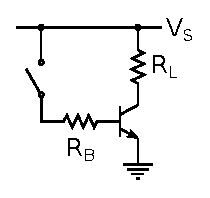
\includegraphics{transistorswitch.eps}
    
  \end{center}
\end{figure}%
\lthtmlfigureZ
\lthtmlcheckvsize\clearpage}

{\newpage\clearpage
\lthtmlinlinemathA{tex2html_wrap_inline1389}%
$R_L$%
\lthtmlindisplaymathZ
\lthtmlcheckvsize\clearpage}

{\newpage\clearpage
\lthtmlinlinemathA{tex2html_wrap_inline1391}%
$R_B$%
\lthtmlindisplaymathZ
\lthtmlcheckvsize\clearpage}

{\newpage\clearpage
\lthtmlinlinemathA{tex2html_wrap_inline1397}%
$\approx V_S$%
\lthtmlindisplaymathZ
\lthtmlcheckvsize\clearpage}

{\newpage\clearpage
\lthtmlinlinemathA{tex2html_wrap_inline1399}%
$\approx 0.25$%
\lthtmlindisplaymathZ
\lthtmlcheckvsize\clearpage}

{\newpage\clearpage
\lthtmlinlinemathA{tex2html_wrap_inline1403}%
$V_S$%
\lthtmlindisplaymathZ
\lthtmlcheckvsize\clearpage}

{\newpage\clearpage
\lthtmlinlinemathA{tex2html_wrap_inline1415}%
$\approx 10~I_C/h_{fe}$%
\lthtmlindisplaymathZ
\lthtmlcheckvsize\clearpage}

\stepcounter{subsection}
{\newpage\clearpage
\lthtmlfigureA{figure568}%
\begin{figure}  \htmlimage{align='center'}{}
  \begin{center}
    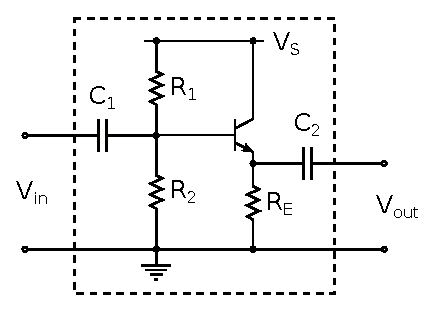
\includegraphics{emitterfollower.eps}
    
  \end{center}
\end{figure}%
\lthtmlfigureZ
\lthtmlcheckvsize\clearpage}

{\newpage\clearpage
\lthtmlinlinemathA{tex2html_wrap_inline1419}%
$A_v \approx 1$%
\lthtmlindisplaymathZ
\lthtmlcheckvsize\clearpage}

{\newpage\clearpage
\lthtmlinlinemathA{tex2html_wrap_inline1421}%
$V_E$%
\lthtmlindisplaymathZ
\lthtmlcheckvsize\clearpage}

{\newpage\clearpage
\lthtmlinlinemathA{tex2html_wrap_inline1425}%
$R_E$%
\lthtmlindisplaymathZ
\lthtmlcheckvsize\clearpage}

{\newpage\clearpage
\lthtmlinlinemathA{tex2html_wrap_inline1435}%
$R_1/R_2$%
\lthtmlindisplaymathZ
\lthtmlcheckvsize\clearpage}

{\newpage\clearpage
\lthtmlinlinemathA{tex2html_wrap_inline1439}%
$V_B \approx V_E + 0.6~\mathrm{V}$%
\lthtmlindisplaymathZ
\lthtmlcheckvsize\clearpage}

{\newpage\clearpage
\lthtmlinlinemathA{tex2html_wrap_inline1441}%
$R_1 || R_2 \approx h_{FE} R_E/ 10$%
\lthtmlindisplaymathZ
\lthtmlcheckvsize\clearpage}

{\newpage\clearpage
\lthtmlinlinemathA{tex2html_wrap_inline1443}%
$C_1$%
\lthtmlindisplaymathZ
\lthtmlcheckvsize\clearpage}

{\newpage\clearpage
\lthtmlinlinemathA{tex2html_wrap_inline1445}%
$C_2$%
\lthtmlindisplaymathZ
\lthtmlcheckvsize\clearpage}

\stepcounter{subsection}
{\newpage\clearpage
\lthtmlfigureA{figure590}%
\begin{figure}  \htmlimage{align='center'}{}
  \begin{center}
    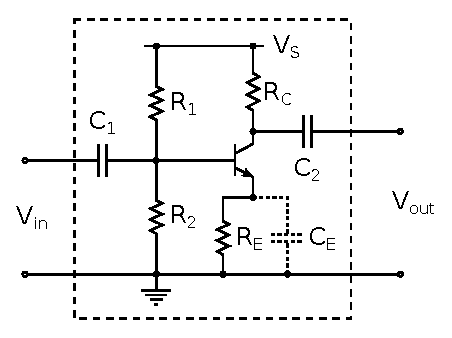
\includegraphics{commonemitter.eps}
    
  \end{center}
\end{figure}%
\lthtmlfigureZ
\lthtmlcheckvsize\clearpage}

{\newpage\clearpage
\lthtmlinlinemathA{tex2html_wrap_indisplay3658}%
$\displaystyle A_v = -\frac{R_C}{R_E}
$%
\lthtmlindisplaymathZ
\lthtmlcheckvsize\clearpage}

{\newpage\clearpage
\lthtmlinlinemathA{tex2html_wrap_inline1447}%
$R_C$%
\lthtmlindisplaymathZ
\lthtmlcheckvsize\clearpage}

{\newpage\clearpage
\lthtmlinlinemathA{tex2html_wrap_inline1453}%
$r_e$%
\lthtmlindisplaymathZ
\lthtmlcheckvsize\clearpage}

{\newpage\clearpage
\lthtmlinlinemathA{tex2html_wrap_inline1457}%
$R_b$%
\lthtmlindisplaymathZ
\lthtmlcheckvsize\clearpage}

{\newpage\clearpage
\lthtmlinlinemathA{tex2html_wrap_inline1463}%
$C_b$%
\lthtmlindisplaymathZ
\lthtmlcheckvsize\clearpage}

{\newpage\clearpage
\lthtmlinlinemathA{tex2html_wrap_inline1465}%
$\approx \frac{R_b}{10}$%
\lthtmlindisplaymathZ
\lthtmlcheckvsize\clearpage}

{\newpage\clearpage
\lthtmlinlinemathA{tex2html_wrap_inline1467}%
$R_E +
  r_e$%
\lthtmlindisplaymathZ
\lthtmlcheckvsize\clearpage}

{\newpage\clearpage
\lthtmlinlinemathA{tex2html_wrap_inline1481}%
$R_1 || R_2 \approx h_{FE} (R_E +
    R_b)/10$%
\lthtmlindisplaymathZ
\lthtmlcheckvsize\clearpage}

{\newpage\clearpage
\lthtmlinlinemathA{tex2html_wrap_inline1489}%
$R_1||R_2$%
\lthtmlindisplaymathZ
\lthtmlcheckvsize\clearpage}

{\newpage\clearpage
\lthtmlinlinemathA{tex2html_wrap_inline1493}%
$R_C||(R_E + R_b)$%
\lthtmlindisplaymathZ
\lthtmlcheckvsize\clearpage}

\stepcounter{section}
{\newpage\clearpage
\lthtmlfigureA{figure622}%
\begin{figure}  \htmlimage{align='center'}{}
  \begin{center}
    \scalebox{0.7}{ 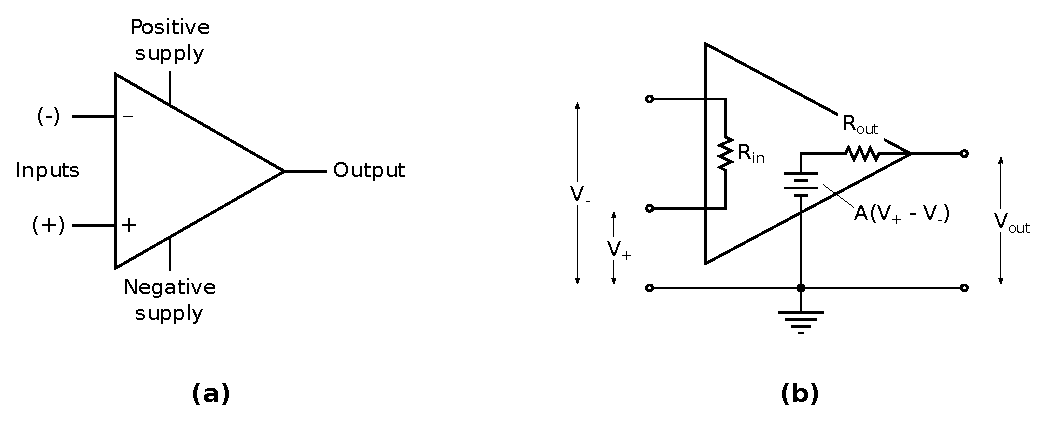
\includegraphics{opamp_model.eps} }
    
  \end{center}
\end{figure}%
\lthtmlfigureZ
\lthtmlcheckvsize\clearpage}

{\newpage\clearpage
\lthtmlinlinemathA{tex2html_wrap_inline1495}%
$V_+ - V_-$%
\lthtmlindisplaymathZ
\lthtmlcheckvsize\clearpage}

{\newpage\clearpage
\lthtmlinlinemathA{tex2html_wrap_inline1499}%
$-V_S \leq V_{out} \leq V_S$%
\lthtmlindisplaymathZ
\lthtmlcheckvsize\clearpage}

{\newpage\clearpage
\lthtmlinlinemathA{tex2html_wrap_inline1503}%
$-V_S < V_{out} < V_S$%
\lthtmlindisplaymathZ
\lthtmlcheckvsize\clearpage}

{\newpage\clearpage
\lthtmlinlinemathA{tex2html_wrap_inline1507}%
$-V_S$%
\lthtmlindisplaymathZ
\lthtmlcheckvsize\clearpage}

{\newpage\clearpage
\lthtmlinlinemathA{tex2html_wrap_inline1509}%
$A = \infty$%
\lthtmlindisplaymathZ
\lthtmlcheckvsize\clearpage}

{\newpage\clearpage
\lthtmlinlinemathA{tex2html_wrap_inline1511}%
$R_{in} = \infty$%
\lthtmlindisplaymathZ
\lthtmlcheckvsize\clearpage}

{\newpage\clearpage
\lthtmlinlinemathA{tex2html_wrap_inline1513}%
$R_{out}
= 0$%
\lthtmlindisplaymathZ
\lthtmlcheckvsize\clearpage}

{\newpage\clearpage
\lthtmlinlinemathA{tex2html_wrap_inline1515}%
$V_+ =
V_-$%
\lthtmlindisplaymathZ
\lthtmlcheckvsize\clearpage}

{\newpage\clearpage
\lthtmlinlinemathA{tex2html_wrap_inline1517}%
$10^3$%
\lthtmlindisplaymathZ
\lthtmlcheckvsize\clearpage}

{\newpage\clearpage
\lthtmlinlinemathA{tex2html_wrap_inline1519}%
$10^5$%
\lthtmlindisplaymathZ
\lthtmlcheckvsize\clearpage}

{\newpage\clearpage
\lthtmlinlinemathA{tex2html_wrap_inline1521}%
$V_+ \approx V_-$%
\lthtmlindisplaymathZ
\lthtmlcheckvsize\clearpage}

{\newpage\clearpage
\lthtmlinlinemathA{tex2html_wrap_inline1523}%
$R_{in} = \infty,~A = \infty,~R_{out} = 0$%
\lthtmlindisplaymathZ
\lthtmlcheckvsize\clearpage}

{\newpage\clearpage
\lthtmlinlinemathA{tex2html_wrap_inline1525}%
$V_+ = V_-,~-V_S < V_{out} < V_S$%
\lthtmlindisplaymathZ
\lthtmlcheckvsize\clearpage}

{\newpage\clearpage
\lthtmlinlinemathA{tex2html_wrap_inline1527}%
$V_+ > V_-~~\Longrightarrow~~V_{out} = V_S$%
\lthtmlindisplaymathZ
\lthtmlcheckvsize\clearpage}

{\newpage\clearpage
\lthtmlinlinemathA{tex2html_wrap_inline1529}%
$V_+ < V_-~~\Longrightarrow~~V_{out} = -V_S$%
\lthtmlindisplaymathZ
\lthtmlcheckvsize\clearpage}

{\newpage\clearpage
\lthtmlinlinemathA{tex2html_wrap_inline1533}%
$10^{12}~\Omega$%
\lthtmlindisplaymathZ
\lthtmlcheckvsize\clearpage}

\stepcounter{subsection}
{\newpage\clearpage
\lthtmlfigureA{figure664}%
\begin{figure}  \htmlimage{align='center'}{}
  \begin{center}
    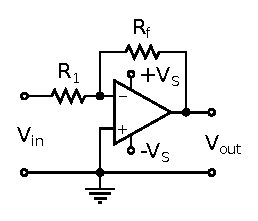
\includegraphics{invertingamp.eps}
    
  \end{center}
\end{figure}%
\lthtmlfigureZ
\lthtmlcheckvsize\clearpage}

{\newpage\clearpage
\lthtmlinlinemathA{tex2html_wrap_inline1539}%
$R_f$%
\lthtmlindisplaymathZ
\lthtmlcheckvsize\clearpage}

{\newpage\clearpage
\lthtmlinlinemathA{tex2html_wrap_indisplay3717}%
$\displaystyle I = \frac{V_{in}}{R_1} = \frac{-V_{out}}{R_f}
$%
\lthtmlindisplaymathZ
\lthtmlcheckvsize\clearpage}

{\newpage\clearpage
\lthtmlinlinemathA{tex2html_wrap_indisplay3719}%
$\displaystyle A_v = -\frac{R_f}{R_1}
$%
\lthtmlindisplaymathZ
\lthtmlcheckvsize\clearpage}

{\newpage\clearpage
\lthtmlinlinemathA{tex2html_wrap_inline1545}%
$R_{oa}||R_f$%
\lthtmlindisplaymathZ
\lthtmlcheckvsize\clearpage}

{\newpage\clearpage
\lthtmlinlinemathA{tex2html_wrap_inline1547}%
$R_{oa}$%
\lthtmlindisplaymathZ
\lthtmlcheckvsize\clearpage}

{\newpage\clearpage
\lthtmlinlinemathA{tex2html_wrap_inline1551}%
$R_f/R_1$%
\lthtmlindisplaymathZ
\lthtmlcheckvsize\clearpage}

\stepcounter{subsection}
{\newpage\clearpage
\lthtmlfigureA{figure696}%
\begin{figure}  \htmlimage{align='center'}{}
  \begin{center}
    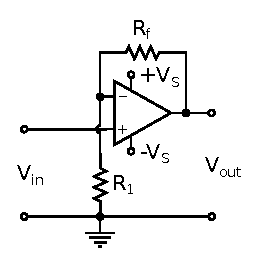
\includegraphics{noninvertingamp.eps}
    
  \end{center}
\end{figure}%
\lthtmlfigureZ
\lthtmlcheckvsize\clearpage}

{\newpage\clearpage
\lthtmlinlinemathA{tex2html_wrap_indisplay3737}%
$\displaystyle V_{in} = \frac{R_1}{R_1 + R_f} V_{out}
$%
\lthtmlindisplaymathZ
\lthtmlcheckvsize\clearpage}

{\newpage\clearpage
\lthtmlinlinemathA{tex2html_wrap_indisplay3739}%
$\displaystyle A_v = 1 + \frac{R_f}{R_1}
$%
\lthtmlindisplaymathZ
\lthtmlcheckvsize\clearpage}

{\newpage\clearpage
\lthtmlinlinemathA{tex2html_wrap_inline1563}%
$R_{oa}||(R_1 + R_f)$%
\lthtmlindisplaymathZ
\lthtmlcheckvsize\clearpage}

\stepcounter{subsection}
{\newpage\clearpage
\lthtmlfigureA{figure729}%
\begin{figure}  \htmlimage{align='center'}{}
  \begin{center}
    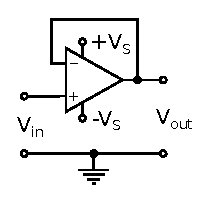
\includegraphics{vfollower.eps}
    
  \end{center}
\end{figure}%
\lthtmlfigureZ
\lthtmlcheckvsize\clearpage}

{\newpage\clearpage
\lthtmlinlinemathA{tex2html_wrap_inline1579}%
$R_1 = \infty$%
\lthtmlindisplaymathZ
\lthtmlcheckvsize\clearpage}

{\newpage\clearpage
\lthtmlinlinemathA{tex2html_wrap_inline1581}%
$R_f = 0$%
\lthtmlindisplaymathZ
\lthtmlcheckvsize\clearpage}

{\newpage\clearpage
\lthtmlinlinemathA{tex2html_wrap_inline1583}%
$A_v = 1$%
\lthtmlindisplaymathZ
\lthtmlcheckvsize\clearpage}

\stepcounter{subsection}
{\newpage\clearpage
\lthtmlfigureA{figure742}%
\begin{figure}  \htmlimage{align='center'}{}
  \begin{center}
    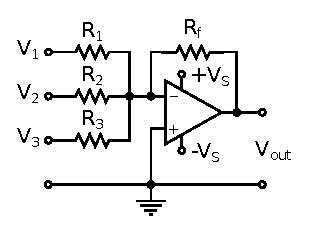
\includegraphics{summingamp.eps}
    
  \end{center}
\end{figure}%
\lthtmlfigureZ
\lthtmlcheckvsize\clearpage}

{\newpage\clearpage
\lthtmlinlinemathA{tex2html_wrap_indisplay3761}%
$\displaystyle I_1$%
\lthtmlindisplaymathZ
\lthtmlcheckvsize\clearpage}

{\newpage\clearpage
\lthtmlinlinemathA{tex2html_wrap_indisplay3763}%
$\displaystyle \frac{V_1}{R_1}$%
\lthtmlindisplaymathZ
\lthtmlcheckvsize\clearpage}

{\newpage\clearpage
\lthtmlinlinemathA{tex2html_wrap_indisplay3764}%
$\displaystyle I_2$%
\lthtmlindisplaymathZ
\lthtmlcheckvsize\clearpage}

{\newpage\clearpage
\lthtmlinlinemathA{tex2html_wrap_indisplay3766}%
$\displaystyle \frac{V_2}{R_2}$%
\lthtmlindisplaymathZ
\lthtmlcheckvsize\clearpage}

{\newpage\clearpage
\lthtmlinlinemathA{tex2html_wrap_indisplay3767}%
$\displaystyle I_3$%
\lthtmlindisplaymathZ
\lthtmlcheckvsize\clearpage}

{\newpage\clearpage
\lthtmlinlinemathA{tex2html_wrap_indisplay3769}%
$\displaystyle \frac{V_3}{R_3}$%
\lthtmlindisplaymathZ
\lthtmlcheckvsize\clearpage}

{\newpage\clearpage
\lthtmlinlinemathA{tex2html_wrap_indisplay3770}%
$\displaystyle I_f$%
\lthtmlindisplaymathZ
\lthtmlcheckvsize\clearpage}

{\newpage\clearpage
\lthtmlinlinemathA{tex2html_wrap_indisplay3772}%
$\displaystyle \frac{V_{out}}{R_f}$%
\lthtmlindisplaymathZ
\lthtmlcheckvsize\clearpage}

{\newpage\clearpage
\lthtmlinlinemathA{tex2html_wrap_indisplay3774}%
$\displaystyle
  I_1 + I_2 + I_3 = I_f
$%
\lthtmlindisplaymathZ
\lthtmlcheckvsize\clearpage}

{\newpage\clearpage
\lthtmlinlinemathA{tex2html_wrap_indisplay3776}%
$\displaystyle
  V_{out} = -\left( \frac{R_1}{R_f} V_1 + \frac{R_2}{R_f} V_2 +
  \frac{R_3}{R_f} V_3 \right)
$%
\lthtmlindisplaymathZ
\lthtmlcheckvsize\clearpage}

{\newpage\clearpage
\lthtmlinlinemathA{tex2html_wrap_inline1589}%
$R_1/R_f$%
\lthtmlindisplaymathZ
\lthtmlcheckvsize\clearpage}

\stepcounter{subsection}
{\newpage\clearpage
\lthtmlfigureA{figure788}%
\begin{figure}  \htmlimage{align='center'}{}
  \begin{center}
    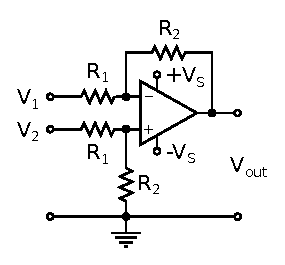
\includegraphics{differenceamp.eps}
    
  \end{center}
\end{figure}%
\lthtmlfigureZ
\lthtmlcheckvsize\clearpage}

{\newpage\clearpage
\lthtmlinlinemathA{tex2html_wrap_indisplay3788}%
$\displaystyle I_1 + I_2 = I_3 + I_4
$%
\lthtmlindisplaymathZ
\lthtmlcheckvsize\clearpage}

{\newpage\clearpage
\lthtmlinlinemathA{tex2html_wrap_indisplay3792}%
$\displaystyle \frac{V_1 - V_-}{R_1}$%
\lthtmlindisplaymathZ
\lthtmlcheckvsize\clearpage}

{\newpage\clearpage
\lthtmlinlinemathA{tex2html_wrap_indisplay3795}%
$\displaystyle \frac{V_2 - V_+}{R_1}$%
\lthtmlindisplaymathZ
\lthtmlcheckvsize\clearpage}

{\newpage\clearpage
\lthtmlinlinemathA{tex2html_wrap_indisplay3798}%
$\displaystyle \frac{V_- - V_{out}}{R_2}$%
\lthtmlindisplaymathZ
\lthtmlcheckvsize\clearpage}

{\newpage\clearpage
\lthtmlinlinemathA{tex2html_wrap_indisplay3799}%
$\displaystyle I_4$%
\lthtmlindisplaymathZ
\lthtmlcheckvsize\clearpage}

{\newpage\clearpage
\lthtmlinlinemathA{tex2html_wrap_indisplay3801}%
$\displaystyle \frac{V_+}{R_2}$%
\lthtmlindisplaymathZ
\lthtmlcheckvsize\clearpage}

{\newpage\clearpage
\lthtmlinlinemathA{tex2html_wrap_indisplay3803}%
$\displaystyle
  V_+ = \frac{R_2}{R_1 + R_2} V_2
$%
\lthtmlindisplaymathZ
\lthtmlcheckvsize\clearpage}

{\newpage\clearpage
\lthtmlinlinemathA{tex2html_wrap_inline1595}%
$V_- = V_+$%
\lthtmlindisplaymathZ
\lthtmlcheckvsize\clearpage}

{\newpage\clearpage
\lthtmlinlinemathA{tex2html_wrap_indisplay3806}%
$\displaystyle V_{out} = - \frac{R_2}{R_1} \left(V_1 - V_2\right)
$%
\lthtmlindisplaymathZ
\lthtmlcheckvsize\clearpage}

{\newpage\clearpage
\lthtmlinlinemathA{tex2html_wrap_inline1603}%
$V_1$%
\lthtmlindisplaymathZ
\lthtmlcheckvsize\clearpage}

{\newpage\clearpage
\lthtmlinlinemathA{tex2html_wrap_inline1605}%
$V_2$%
\lthtmlindisplaymathZ
\lthtmlcheckvsize\clearpage}

\stepcounter{subsection}
{\newpage\clearpage
\lthtmlfigureA{figure828}%
\begin{figure}  \htmlimage{align='center'}{}
  \begin{center}
    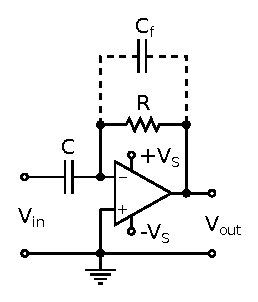
\includegraphics{differentiator.eps}
    
  \end{center}
\end{figure}%
\lthtmlfigureZ
\lthtmlcheckvsize\clearpage}

{\newpage\clearpage
\lthtmlinlinemathA{tex2html_wrap_inline1607}%
$C_f
< C$%
\lthtmlindisplaymathZ
\lthtmlcheckvsize\clearpage}

{\newpage\clearpage
\lthtmlinlinemathA{tex2html_wrap_inline1609}%
$C_f$%
\lthtmlindisplaymathZ
\lthtmlcheckvsize\clearpage}

{\newpage\clearpage
\lthtmlinlinemathA{tex2html_wrap_indisplay3820}%
$\displaystyle
  V_{out} = - IR
$%
\lthtmlindisplaymathZ
\lthtmlcheckvsize\clearpage}

{\newpage\clearpage
\lthtmlinlinemathA{tex2html_wrap_indisplay3822}%
$\displaystyle V_{in} = \frac{Q}{C}
$%
\lthtmlindisplaymathZ
\lthtmlcheckvsize\clearpage}

{\newpage\clearpage
\lthtmlinlinemathA{tex2html_wrap_indisplay3825}%
$\displaystyle
  I \equiv \frac{dQ}{dt}
$%
\lthtmlindisplaymathZ
\lthtmlcheckvsize\clearpage}

{\newpage\clearpage
\lthtmlinlinemathA{tex2html_wrap_indisplay3827}%
$\displaystyle
  V_{out} = - RC \frac{d V_{in}}{dt}
$%
\lthtmlindisplaymathZ
\lthtmlcheckvsize\clearpage}

{\newpage\clearpage
\lthtmlinlinemathA{tex2html_wrap_inline1617}%
$RC$%
\lthtmlindisplaymathZ
\lthtmlcheckvsize\clearpage}

\stepcounter{subsection}
{\newpage\clearpage
\lthtmlfigureA{figure865}%
\begin{figure}  \htmlimage{align='center'}{}
  \begin{center}
    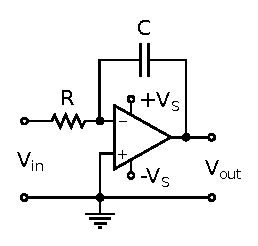
\includegraphics{integrator.eps}
    
  \end{center}
\end{figure}%
\lthtmlfigureZ
\lthtmlcheckvsize\clearpage}

{\newpage\clearpage
\lthtmlinlinemathA{tex2html_wrap_indisplay3838}%
$\displaystyle
  I = \frac{V_{in}}{R}
$%
\lthtmlindisplaymathZ
\lthtmlcheckvsize\clearpage}

{\newpage\clearpage
\lthtmlinlinemathA{tex2html_wrap_indisplay3840}%
$\displaystyle
  V_{out} = -\frac{Q}{C}
$%
\lthtmlindisplaymathZ
\lthtmlcheckvsize\clearpage}

{\newpage\clearpage
\lthtmlinlinemathA{tex2html_wrap_inline1621}%
$I \equiv dQ/dt$%
\lthtmlindisplaymathZ
\lthtmlcheckvsize\clearpage}

{\newpage\clearpage
\lthtmlinlinemathA{tex2html_wrap_indisplay3843}%
$\displaystyle
  Q = \int dQ = \frac{1}{R} \int V_{in} \, dt + \mathrm{constant}
$%
\lthtmlindisplaymathZ
\lthtmlcheckvsize\clearpage}

{\newpage\clearpage
\lthtmlinlinemathA{tex2html_wrap_indisplay3845}%
$\displaystyle
  V_{out} = - \frac{1}{RC} \int V_{in} \, dt + C
$%
\lthtmlindisplaymathZ
\lthtmlcheckvsize\clearpage}

\appendix
\stepcounter{section}
{\newpage\clearpage
\lthtmlfigureA{figure909}%
\begin{figure}  \htmlimage{align='center'}{}
  \begin{center}
    \scalebox{0.8}{
      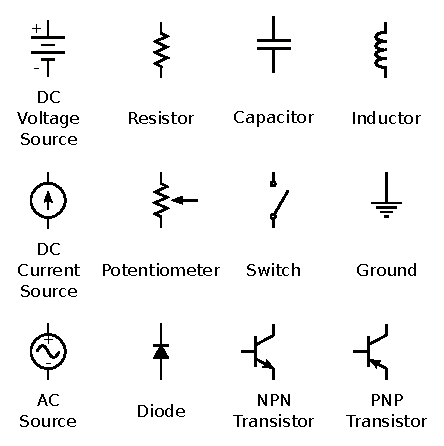
\includegraphics{schematic.eps}
    }
   \end{center}
  
\end{figure}%
\lthtmlfigureZ
\lthtmlcheckvsize\clearpage}

{\newpage\clearpage
\lthtmlpictureA{tex2html_wrap3856}%
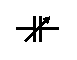
\includegraphics{var_capacitor.eps}%
\lthtmlpictureZ
\lthtmlcheckvsize\clearpage}

{\newpage\clearpage
\lthtmlfigureA{figure924}%
\begin{figure}  \htmlimage{align='center'}{}
  \begin{center}
    \scalebox{0.8}{
      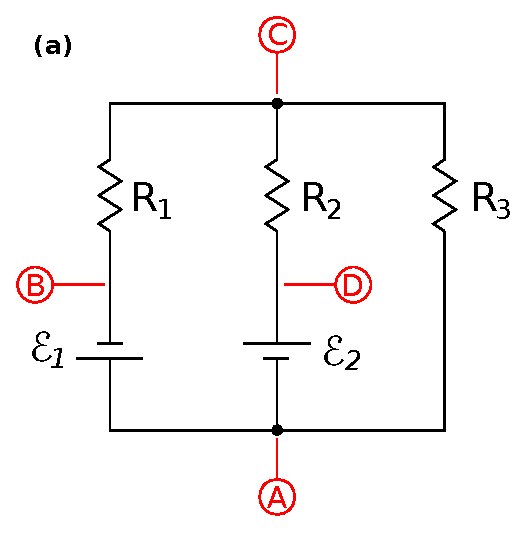
\includegraphics{schematic_example.eps}
    }\\
    \vspace{12 pt}
    \scalebox{0.8}{
      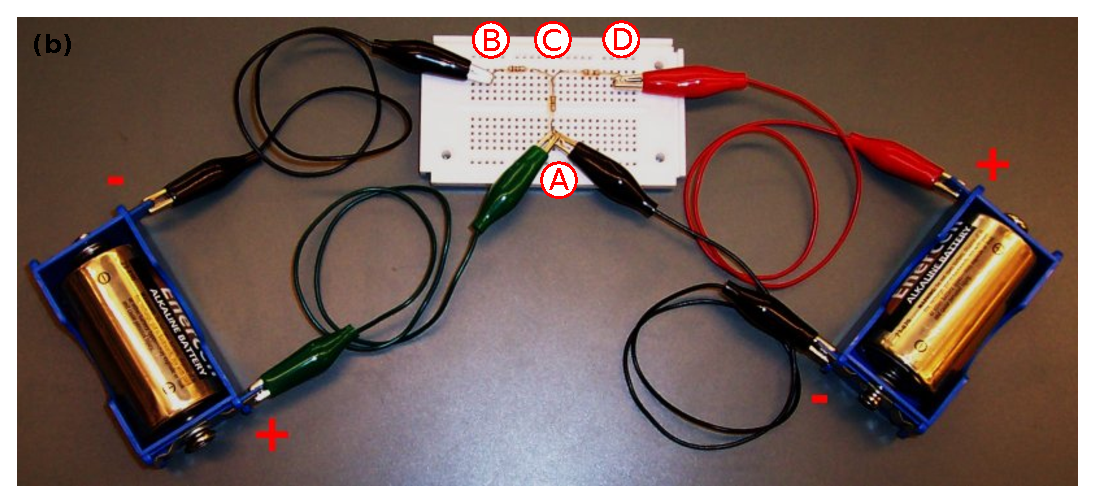
\includegraphics{schematic_example_image.eps}
    }
   \end{center}
  
\end{figure}%
\lthtmlfigureZ
\lthtmlcheckvsize\clearpage}

\stepcounter{section}
{\newpage\clearpage
\lthtmlfigureA{figure946}%
\begin{figure}  \htmlimage{align='center'}{}
  \begin{center}
    \scalebox{0.5}{
      \includegraphics{breadboard.eps}
    }
    
  \end{center}
\end{figure}%
\lthtmlfigureZ
\lthtmlcheckvsize\clearpage}

\stepcounter{section}
{\newpage\clearpage
\lthtmlfigureA{figure959}%
\begin{figure}  \htmlimage{align='center'}{}
  \begin{center}
    %% Latex2html doesn't recognize the colortabl package, so...
    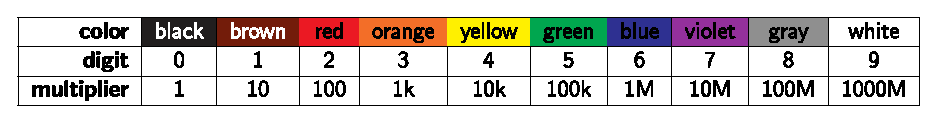
\includegraphics{resistor_color_codes.eps}
    \begin{eqnarray*}
      R = [\mathrm{band 1}][\mathrm{band 2}] 
      \times 10^{[\mathrm{band 3}]} & \pm & 5\%~(\mathrm{gold})\\
      & \pm & 10\%~(\mathrm{silver})\nonumber
    \end{eqnarray*}
    
  \end{center}
\end{figure}%
\lthtmlfigureZ
\lthtmlcheckvsize\clearpage}

{\newpage\clearpage
\lthtmlinlinemathA{tex2html_wrap_inline1633}%
$R = 64
\times 10^{2}~\Omega = 64 \times 100~\Omega = 6400~\Omega$%
\lthtmlindisplaymathZ
\lthtmlcheckvsize\clearpage}

{\newpage\clearpage
\lthtmlinlinemathA{tex2html_wrap_inline1635}%
$\pm 320~\Omega$%
\lthtmlindisplaymathZ
\lthtmlcheckvsize\clearpage}

\stepcounter{section}
{\newpage\clearpage
\lthtmlfigureA{figure978}%
\begin{figure}  \htmlimage{align='center'}{}
  \begin{center}
    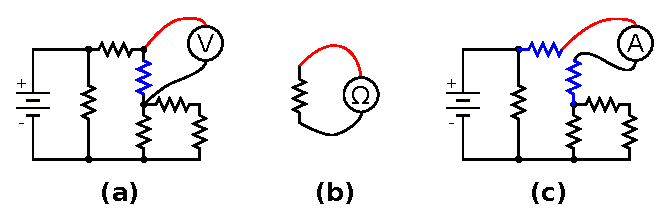
\includegraphics{dmm.eps}
\par
  \end{center}
\end{figure}%
\lthtmlfigureZ
\lthtmlcheckvsize\clearpage}

\stepcounter{subsection}
\stepcounter{subsection}
\stepcounter{subsection}
\stepcounter{section}
{\newpage\clearpage
\lthtmlinlinemathA{tex2html_wrap_inline1641}%
$Thing_1$%
\lthtmlindisplaymathZ
\lthtmlcheckvsize\clearpage}

{\newpage\clearpage
\lthtmlinlinemathA{tex2html_wrap_inline1643}%
$Thing_2$%
\lthtmlindisplaymathZ
\lthtmlcheckvsize\clearpage}

{\newpage\clearpage
\lthtmlinlinemathA{tex2html_wrap_indisplay3886}%
$\displaystyle dB = 10 \log \left( \frac{\mathrm{Thing_2}}{\mathrm{Thing_1}} \right)
$%
\lthtmlindisplaymathZ
\lthtmlcheckvsize\clearpage}

{\newpage\clearpage
\lthtmlinlinemathA{tex2html_wrap_inline1645}%
$\mathrm{Thing_2}$%
\lthtmlindisplaymathZ
\lthtmlcheckvsize\clearpage}

{\newpage\clearpage
\lthtmlinlinemathA{tex2html_wrap_inline1647}%
$10^8$%
\lthtmlindisplaymathZ
\lthtmlcheckvsize\clearpage}

{\newpage\clearpage
\lthtmlinlinemathA{tex2html_wrap_inline1649}%
$\mathrm{Thing_1}$%
\lthtmlindisplaymathZ
\lthtmlcheckvsize\clearpage}

{\newpage\clearpage
\lthtmlinlinemathA{tex2html_wrap_inline1659}%
$10^{-12}$%
\lthtmlindisplaymathZ
\lthtmlcheckvsize\clearpage}

{\newpage\clearpage
\lthtmlinlinemathA{tex2html_wrap_inline1661}%
$^2$%
\lthtmlindisplaymathZ
\lthtmlcheckvsize\clearpage}

{\newpage\clearpage
\lthtmlinlinemathA{tex2html_wrap_indisplay3897}%
$\displaystyle 10 \log \left( \frac{P_{out}}{P_{in}} \right)
= 10 \log \left( \frac{1}{2} \right) = 10 (-0.3010) = -3.01
$%
\lthtmlindisplaymathZ
\lthtmlcheckvsize\clearpage}

{\newpage\clearpage
\lthtmlinlinemathA{tex2html_wrap_inline1663}%
$A_v = |V_{out}|/|V_{in}|$%
\lthtmlindisplaymathZ
\lthtmlcheckvsize\clearpage}

{\newpage\clearpage
\lthtmlinlinemathA{tex2html_wrap_inline1665}%
$1/\sqrt{2}$%
\lthtmlindisplaymathZ
\lthtmlcheckvsize\clearpage}

{\newpage\clearpage
\lthtmlinlinemathA{tex2html_wrap_inline1667}%
$|A_v|/|A_{v_{max}}|$%
\lthtmlindisplaymathZ
\lthtmlcheckvsize\clearpage}


\end{document}
